\documentclass{standalone}
\usepackage{pgfplots}
\pgfplotsset{compat=newest}

\begin{document}
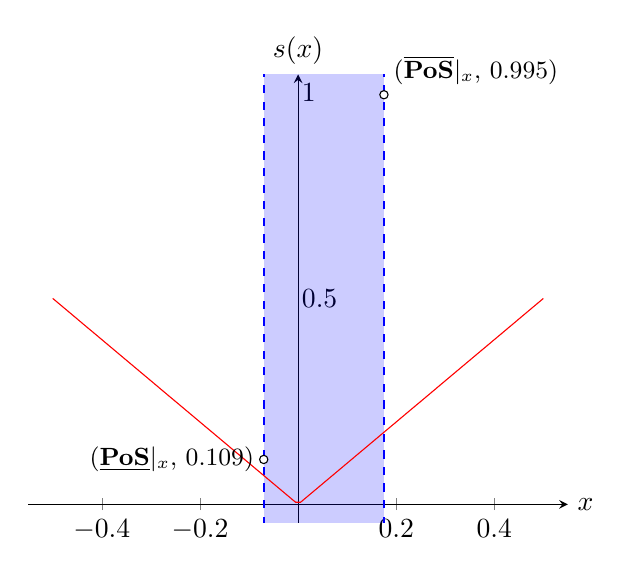
\begin{tikzpicture}
  \begin{axis}[
      axis lines = middle,
      xlabel = $x$,
      xlabel style ={anchor=west},
      ylabel = $\text{s}(x)$,
      ylabel style = {anchor=south},
      ytick distance = 0.5,
      ytick pos = right,
      enlargelimits = 0.05,
  ]
  % PoS footprint
  \fill[blue, opacity=0.2] (axis cs:-0.07,-0.05) rectangle (axis cs:0.175,1.05);
  \draw[blue, thick, dashed] (axis cs:-0.07,-0.05) -- (axis cs:-0.07,1.05);
  \draw[blue, thick, dashed] (axis cs:0.175,-0.05) -- (axis cs:0.175,1.05);

  % abs
  \addplot [
      domain=-0.5:0.5,
      samples=100,
      color=red,
      ]
      {x^2^(1/2)};
  % example marker
  \addplot[
    only marks,
    mark=*,
    mark options={scale=0.75,fill=white},
    point meta=explicit symbolic,
    nodes near coords,
    nodes near coords style={anchor=south west},
    every node near coord/.append style={font=\small},
    ] coordinates {
      (0.175, 0.9948) [($\overline{\textbf{PoS}}|_x$, 0.995)]
    };
  \addplot[
    only marks,
    mark=*,
    mark options={scale=0.75,fill=white},
    point meta=explicit symbolic,
    nodes near coords,
    nodes near coords style={anchor=east},
    every node near coord/.append style={font=\small},
    ] coordinates {
      (-0.07, 0.109) [($\underline{\textbf{PoS}}|_x$, 0.109)]
    };
  \end{axis}
\end{tikzpicture}
\end{document}
